EPCON is a startup company that works in multiple fields of digital social or medical software like epidemics and NGO support. This project from EPCON was focused on computer-aided diagnosis, specifically for tuberculosis, and for under-developed world regions.

\section{Problem domain}

We were told about the problem and all the details when we first met with EPCON in Belgium. During this meeting they showed us their API and a demo web application they had built that connected to this API. It allowed users to upload a pulmonary X-ray image and to get an output image with the areas where signs were found and a likelihood of tuberculosis. \cite{Biometrics}
\\
See the screenshot of the app below:
\\ \\

\begin{figure}[H]
	\centering
	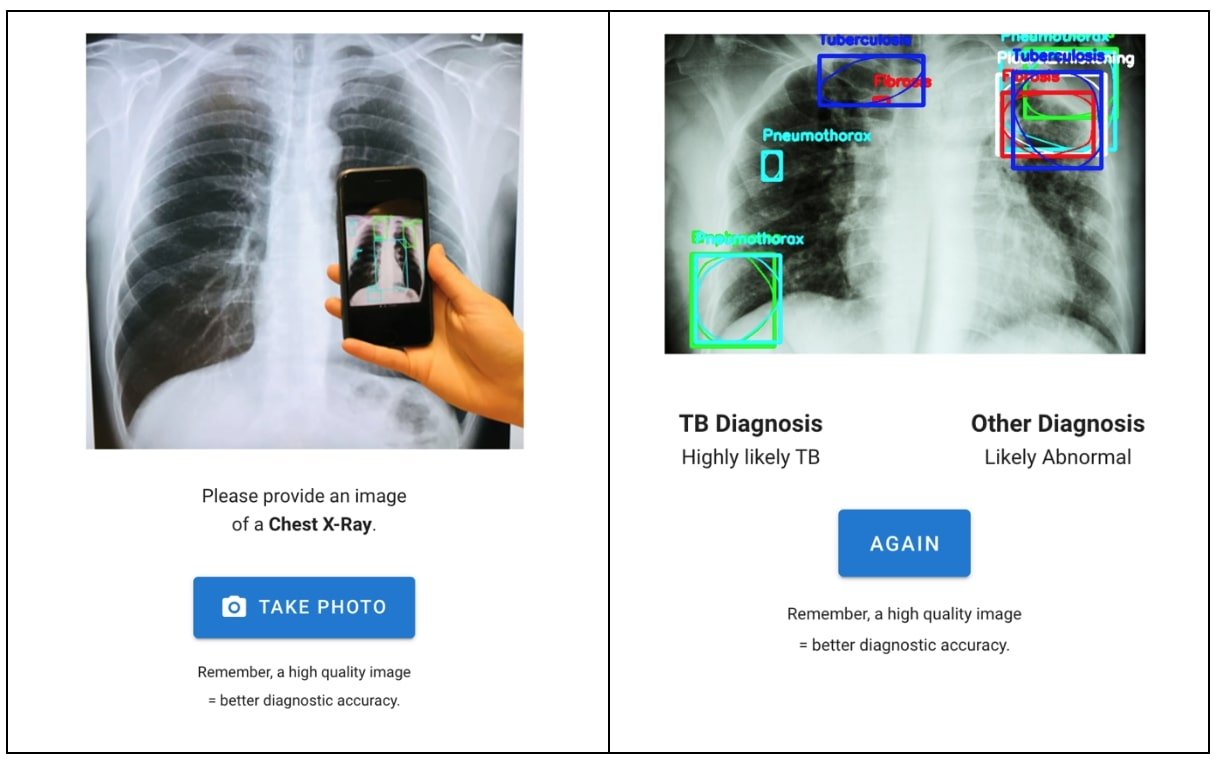
\includegraphics[width=0.8\linewidth]{pesti-report/images/epcon-web-app.jpg}
	\caption{EPCON demo web application}
	\label{fig:epcon-web-app}
\end{figure}

\\

This demo application had three main problems:

\begin{itemize}
\item
It connected directly with the artificial intelligence API, which made all the requests very slow
\item
It didn't use the latest symptoms payload they have added to the API
\item
It didn't persist data
\end{itemize}

So, our project was to build a system that would consume this machine learning API they have created that addressed all the listed problems and more.
\\ \\
EPCON wanted the app to be free to use for anyone, but they also wanted to have a registration system for doctors who wanted to persist all their screenings and patients. The app should allow doctors to manage patients and screen their respective X-rays.

\section{Functional requirements}

One of our first approaches during the first meeting was to try to define user-stories and write all of them down.

\\ \\
\begin{figure}[H]
	\centering
	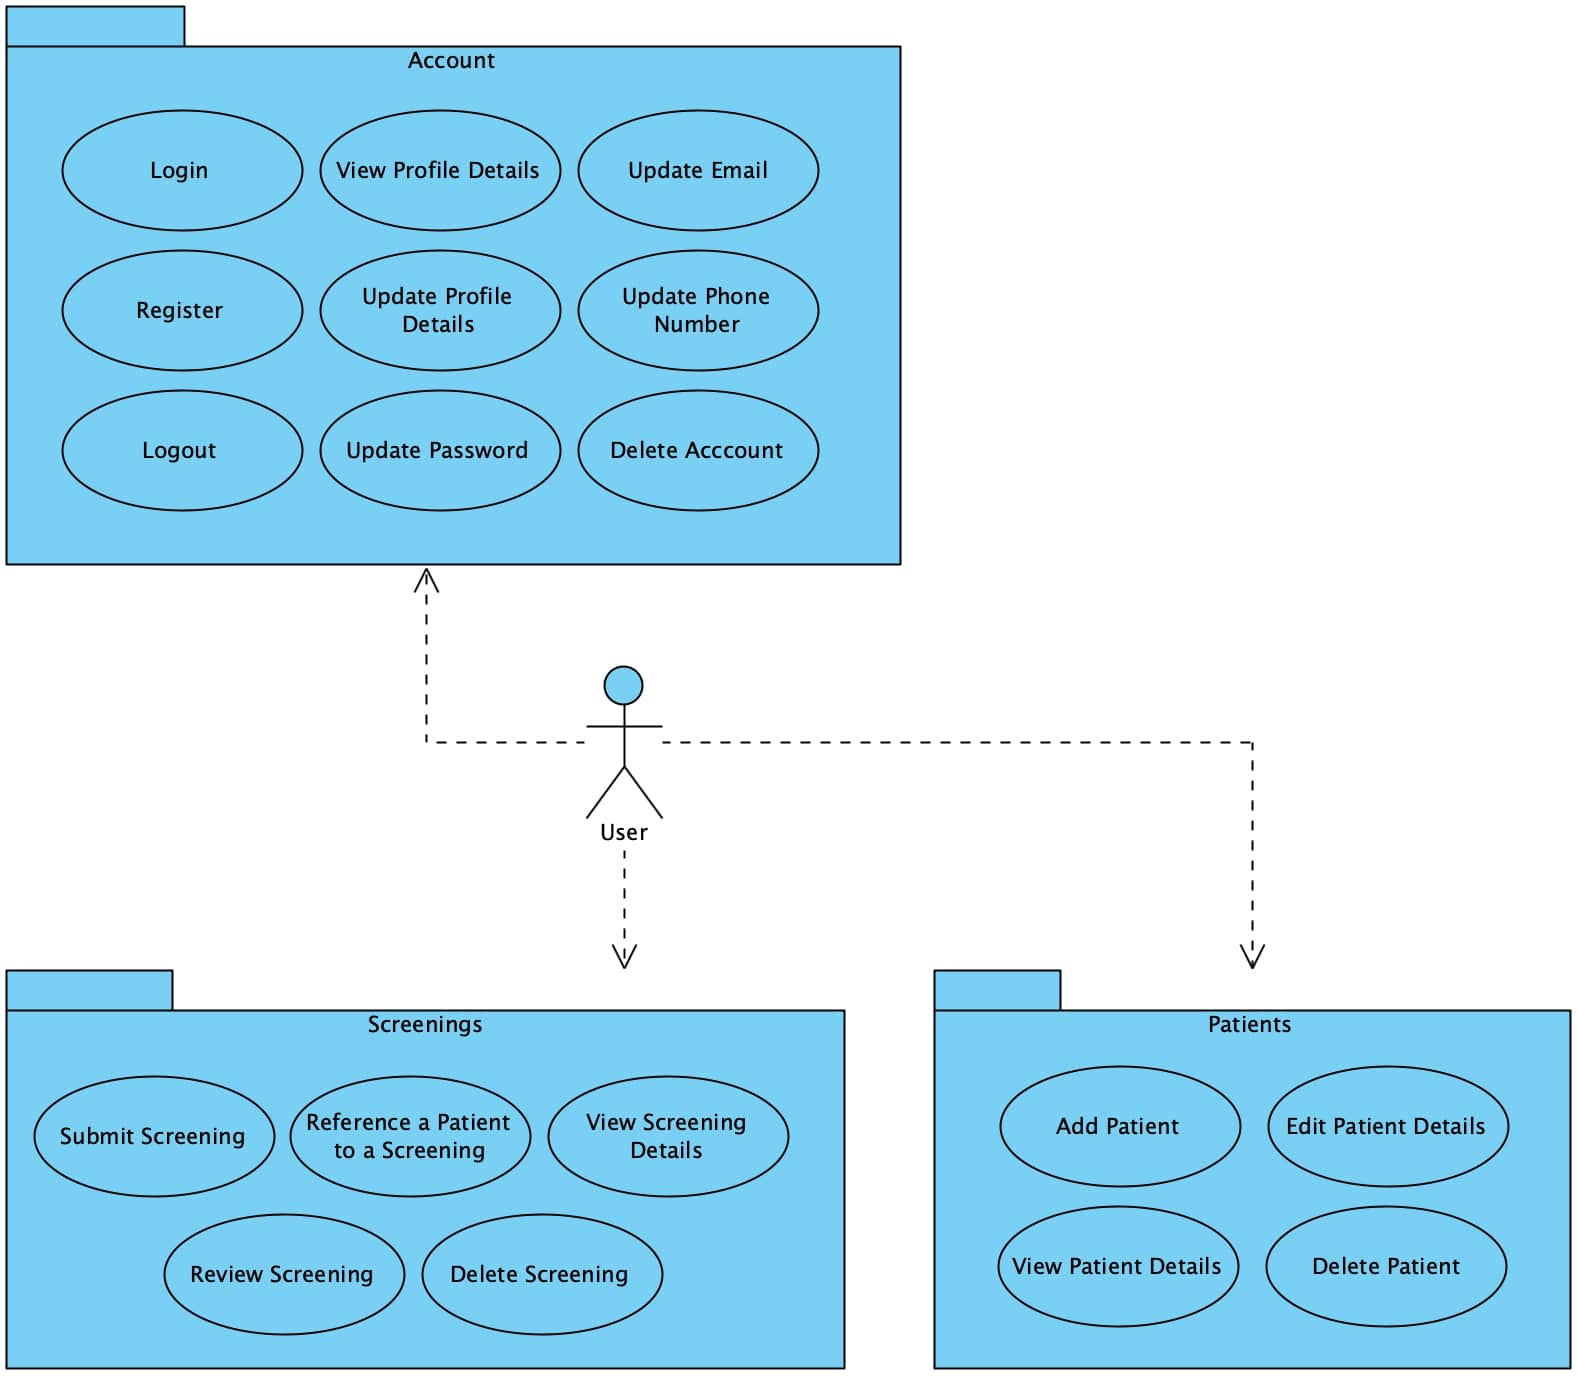
\includegraphics[width=1.0\linewidth]{pesti-report/images/use-case-diagram.jpg}
	\caption{Use case diagram}
	\label{fig:use-case-diagram}
\end{figure}

\\
Here are the use cases we collected:

\begin{itemize}
\item
A user can register using email, password and phone number
\item
A user can login using email and password
\item
A logged user can logout
\item
A logged user can view his/her profile
\item
A logged user can edit his/her profile (name, city, country and bio)
\item
A logged user can edit his/her password
\item
A logged user can edit his/her phone number
\item
A logged user can edit his/her email address
\item
A logged user can delete his/her account
\item
A user can submit a screening for diagnosis
\item
A user can view the diagnosis of a specific screening
\item
A user can view the list of his/her screenings
\item
A user can review a diagnosed screening
\item
A user can delete a specific screening
\item
A logged user can add a patient
\item
A logged user can view the list of his/her patients
\item
A logged user can view a specific patient details
\item
A logged user can edit a patient details(name, sex and year of birth)
\item
A logged user can delete a specific patient
\item
A logged user can reference a patient when submitting a screening
\item
A user can read the version changelog
\item
A user can read the about statement
\item
A user can read the terms and conditions
\item
A user can read the privacy policy
\item
A user can read the cookie policy
\end{itemize}

\section{Domain modeling}

The first step was to identify the different domains we would be working with. This was a time-consuming process because all of us were completely new to this computer-aided diagnosis area and also because all of us came from different countries and were speaking a non-native language. Nevertheless, we came up with these three different domains:

\begin{itemize}
\item
User
\item
Patient
\item
Screening
\end{itemize}

A \textbf{user} is anyone who is using the app. The app is targeted to be use by doctors, healthcare professionals or medical students, but it is free and open to anyone, so we thought it would be better to abstract from the concept of doctor.
\\ \\
A \textbf{patient} is a record added and persisted by a user and can be referenced on a screening.
\\ \\
A \textbf{screening} is an attempt to diagnose an X-ray pulmonary image.


\\ \\
\begin{figure}[!h]
	\centering
	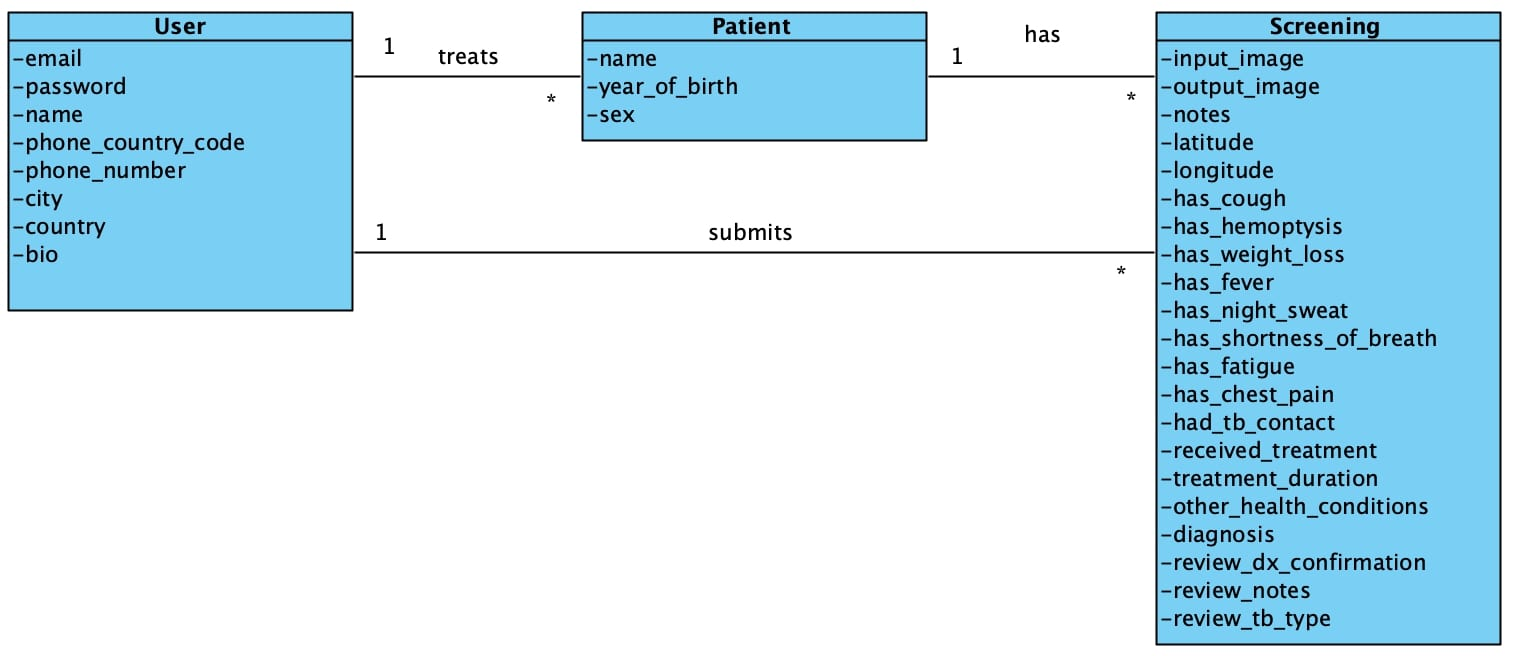
\includegraphics[width=1.0\linewidth]{pesti-report/images/domain-model.jpg}
	\caption{Domain model}
	\label{fig:domain-model}
\end{figure}
\\
